El presente trabajo pretende exhibir un modelo matemático en EDP(Ecuaciones en derivadas parciales) que pueda predecir el crecimiento de un tumor cerebral a lo largo del tiempo; para dar la expresión explícita del modelo (ecuaciones), necesitamos partir de algunos conceptos y modelos previos.\\

%%%%%%%%%%%%%%%%%%%%%%%%%%%%%%%%%%%%%%%%%%%%%%%%%%%%%%%%%%%%%%%%%%%%%%%%%%%%%%%%%%%%%%%%%%%%%%% 
\section{¿Qué es el cáncer?}

\subsection{Antecedentes}

En la antig\"uedad el hombre no estaba menos preocupado por la prevención y cura de enfermedades como ocurre ahora; sin embargo,
diversas entidades como cultos y santuarios, e incluso profesionales dedicados a la salud punteaban los paisajes espirituales, físicos y
profesionales del mundo antiguo.\\

Especialidades de distintas ramas como arqueología, paleontología y paleomedicina han descubierto en diversas culturas restos óseos humanos fosilizados afectados por el cáncer y han determinado su antig\"uedad en miles de años atrás mediante carbono $14$.\\

Ese descubrimiento fue importante pues nos hace asegurar que incluso en el pasado ha existido el cáncer y que en la actualidad se ha configurado en la principal causa de muerte en todo el mundo.

\subsection{¿Qué sabemos del cáncer en la actualidad?}

Sabemos que nuestro organismo está constituido por un gran número de células y que estas son la unidad anatómica fundamental funcional de todos los seres vivos y además su composición es compleja y única, como por ejemplo: el ADN y el ARN.\\

Cada una de las células crece y se divide de manera coordinada y ordenada; sin embargo, algunas veces este proceso se descontrola y el material genético contenido en el ADN se daña o se altera, provocando así mutaciones irreversibles que afectan en el crecimiento y la división normal de las células.\\

Cuando esto último sucede, las células no mueren cuando deberían morir, y se forman células nuevas a pesar de que el cuerpo no las necesita y estas forman una masa de tejido a la que se le llama \textbf{tumor}.

\subsection{Definición}

Se le llama \textbf{cáncer} cuando el tumor es maligno y tiene la capacidad de invasión, infiltración y de producir metástasis a lugares distantes del tumor primario. No obstante, no todos los tumores son cancerosos, entre ellas tenemos:
 
\begin{itemize}
	\item \textbf{Tumores benignos}: Son aquellos que pueden extirparse y en la mayoría de los casos no vuelven a aparecer. Las células no se diseminan a otras partes del cuerpo.
	\item \textbf{Tumores malignos}: Son aquellos en las que las células pueden invadir tejidos cercanos y diseminarse a otras partes del cuerpo.
\end{itemize}

Al proceso en el que las células cancerosas se desprenden del tumor original y viajan a través de la sangre o el sistema linfático y forman un tumor nuevo en otros órganos o tejidos se le llama \textbf{metástasis}.
\subsection{Causas}

El proceso por el cual se produce el cáncer es causado por anormalidades en el material genético de las células. Estas anormalidades pueden ser ocasionadas por:

\begin{itemize}
	\item Agentes carcinógenos como las irradiaciones. 
	\item Algunos productos químicos como el humo del tabaco y el humo de leña.
	\item Por agentes infecciosos como el VIH y el de la hepatitis B.
	\item Anormalidades genéticas adquiridas durante la replicación del ADN.
\end{itemize} 
\subsection{Clasificación}

Por lo general el cáncer se clasifica según los órganos o tejidos en donde se presenta y también se describe según el tipo de célula por el que está formado.

\begin{itemize}
	\item \textbf{Carcinoma}: cáncer que empieza en la piel o en los tejidos que cubren órganos internos.
	\item \textbf{Sarcoma}: cáncer que empieza en el hueso, cartílago, grasa, músculo o vasos sanguineos.
	\item \textbf{Leucemia}: cáncer que empieza en el tejido en el que se forma la sangre, como la médula ósea.
	\item \textbf{Linfoma y mielioma}: cáncer que empieza en las células del sistema inmunitario
	\item \textbf{Cáncer del sistema nervioso central}: cáncer que empieza en los tejidos del cerebro y la médula espinal.
\end{itemize}

Los cinco tipos de cáncer que causan un mayor número de fallecimientos son los siguientes:

\begin{itemize}
	\item Pulmonar
	\item Hepático
	\item Colorrectal
	\item Gástrico
	\item Mamario
\end{itemize}

\subsection{Tumores cerebrales}

Estos tumores se pueden originar a partir de las células cerebrales, las membranas alrededor del cerebro, nervios o glandulas. Los tumores pueden destruir directamente células cerebrales o provocarles daño produciendo inflamación, ejerciendo presión sobre otras partes del cerebro e incrementando la presión intracraneal.\\

Los tumores cerebrales pueden ocurrir a cualquier edad, pero muchos de ellos son más comunes en un grupo de edad en particular. Por ejemplo, en los adultos, los gliomas y los meningiomas son los más comunes.\\

Los \textit{meningiomas} son muy frecuentes y por lo general benignos.No obstante pueden causar serias complicaciones e inluso la muerte debido a su tamaño y localización.\\

Por el contrario los \textit{gliomas},a pesar de que apenas metastatizan, rara vez se pueden curar. Surgen a partir de las células gliales,es decir, células del sistema nervioso central que desempeñan de forma principal, la función de soporte de las neuronas e intervienen activamente en el procesamiento cerebral de la información en el organismo. Son clasificados de acuerdo a su grado, y del cual depende que se augure un mejor o un peor pronóstico, siendo éste por lo general malo para pacientes con gliomas de alto grado.\\

Esta presente investigación tiene como objetivo encontrar una ecuación en derivadas parciales con las condiciones necesarias que modele en concreto los gliomas y resolverla empleando el método numérico adecuado.\\

\begin{figure}[H]
	\centering
	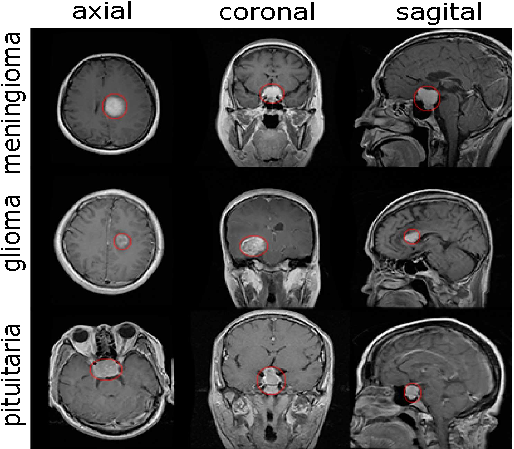
\includegraphics[scale=1.2]{marcoteorico/tumorcerebral.pdf}			
	\caption{{\small {\footnotesize Representación de imágenes de resonancia magnética (MRI) normalizadas que muestran diferentes tipos de tumores en diferentes planos. En las imágenes, el tumor está marcado con un contorno rojo. El ejemplo se da para cada tipo de tumor en cada uno de los planos.}}}
\end{figure}

\newpage
%%%%%%%%%%%%%%%%%%%%%%%%%%%%%%%%%%%%%%%%%%%%%%%%%%%%%%%%%%%%%%%%%%%%%%%%%%%%%%%%%%%%%%%%%%%%%%%%
\section{Ecuación de Reacción-Difusión.}\label{cap: Ec Re Dif}
Estas ecuaciones son importantes en derivadas parciales e implican la combinación de dos procesos diferentes: \textit{reacción} y \textit{difusión}. Empecemos definiendo estos dos conceptos:
\begin{itemize}
	\item \textbf{Difusión}: Es la tendencia de las moléculas a moverse desde zonas de alta concentración hacia zonas de baja concentración.
	\item \textbf{Reacción}: Se entiende como el cambio de estado de las partículas debido por ejemplo a interacciones o de manera espontánea.
\end{itemize}
Estas ecuaciones se sitúan en el campo del Modelado Matemático de Sistemas Biológicos, y se debe tener en cuenta que este modelo surge para intentar describir un medio(sistema) que ignora por completo el efecto de las fluctuaciones internas(algo común en cualquier sistema discreto). A pesar de ello, tales fluctuaciones pueden provocar cambios drásticos en la dinámica, lo que ocasiona una ruptura de las aproximaciones que se obtengan del sistema. Los casos más complejos, se han estudiado en trabajos que incorporan métodos estocásticos.\\

Cabe mencionar que este modelo se ha estudiado sobre todo en dominios espaciales estáticos, sin embargo en los sistemas biológicos es común encontrar dominios en crecimiento; en particular el interés de los dominios en crecimiento se hace evidente en la biología del desarrollo, donde una característica común de los sistemas estudiados es su tamaño dependiente del sistema.\\

Por todo lo expuesto anteriormente, en años recientes, este modelo para dominios en crecimiento viene siendo objeto de gran interés en investigación biológica.\\

Esta ecuación comprende dos factores importantes, uno de difusión y otro de reacción, y el modelo es el siguiente:

\begin{equation}
	\label{ReaccionDifusion1}
	{ u }_{ t }=d\triangle u+f(u)
\end{equation}

\vspace{0.2cm}
Donde:

\begin{itemize}
	\item $u(x,t)$ es la variable de estado y describe la densidad(concentración) de una sustancia(población) en la posición $ x\in \Omega\subset { \mathbb{R} }^{ n }$ y en el instante $t $. (Tener en cuenta que $\Omega$ es un conjunto abierto). Además el operador $ \triangle $ es el Laplaciano.
	\item El factor $d\triangle u $ describe la difusión del sistema, siendo $d$ el coeficiente de difusión.
	\item El factor $f(u)$ es una función suave $f:\mathbb{R}\rightarrow \mathbb{R} $, y este describe el proceso con el que realmente cambia $u$; es decir, podría ocurrir un proceso como nacimiento, muerte,reacción química, etc.
\end{itemize}

Entendiéndose en términos más simples, el \textbf{factor de difusión} nos dice qué tanto cambia el espacio (expande o contrae) y \textbf{el factor de reacción} nos da información acerca de lo que pasa dentro del espacio y los cambios que ocurren en él. Obteniendo así información del sistema completo.\\

Este modelo se puede llevar a sistemas más complejos en los que el factor de Reacción no solo dependa de $u$, sino también de su derivada($ \nabla u$) o incluso de la variable espacial $x$, en tal caso tendríamos lo siguiente:

\begin{equation}
	\label{ReaccionDifusion2}
	 u_{ t }=d\triangle u + f(x,u,\nabla u)
\end{equation}

\vspace{0.2cm}
Sin embargo, para este trabajo solo tomaremos la idea de la ecuación (\ref{ReaccionDifusion1})
%%%%%%%%%%%%%%%%%%%%%%%%%%%%%%%%%%%%%%%%%%%%%%%%%%%%%%%%%%%%%%%%%%%%%%%%%%%%%%%%%%%%%%%%%%%%%%%
\section{Modelo logístico de poblaciones.}\label{cap:mod log pob}
Los dos modelos más simples de crecimiento poblacional utilizan ecuaciones determinísticas(ecuaciones que no consideran los eventos aleatorios) para describir la tasa de cambio en el tiempo de la población. El primero de estos , \textbf{crecimiento exponencial}, describe poblaciones que incrementan su número sin ningún límite; sin embargo esto solo es posible  únicamente cuando hay disponible una cantidad infinita de recursos, lo cual no ocurre en la realidad ya que si los individuos se incrementan los recursos se terminaran, la tasa de crecimiento disminuirá. Eventualmente la tasa de crecimiento alcanzará una asíntota o se estabilizará. Este tamaño de la población, que esta determinado por un tamaño máximo de población que un ambiente puede mantener se llama \textbf{capacidad de carga}. Por tanto en este segundo caso se dice que la población tiene un \textbf{crecimieno logístico}. 

\begin{center}
	\begin{figure}[H]
		\centering
		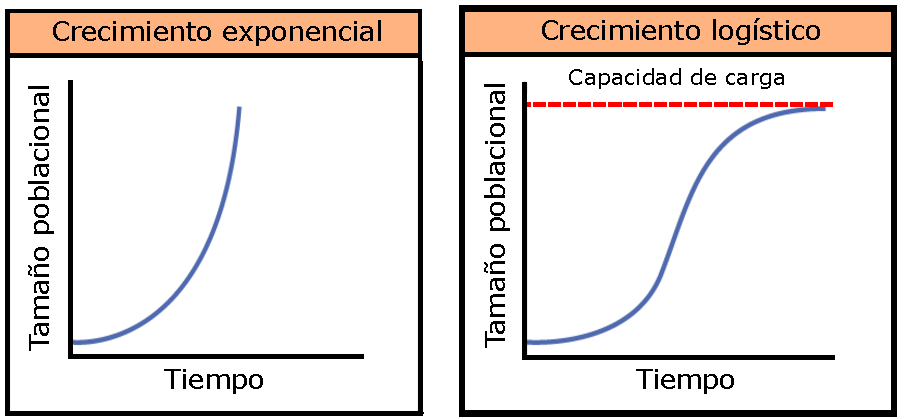
\includegraphics[scale=1]{marcoteorico/crecimientologistico.pdf}			
		\caption{{\small {\footnotesize Dos modelos básicos que describen el crecimiento poblacional}}}
	\end{figure}
\end{center}

Si bien, existen muchos modelos matemáticos más sofisticados sobre poblaciones de organismos biológicos, el siguinte modelo en particular será de sumo interés pues será este quien nos conducirá a la ecuación medular de este trabajo(Ecuación de Fisher-Kolmogorov)\\

Si usamos un modelo poblacional, en el que se asume que los recursos son limitados tendremos el siguiente sistema:

\begin{equation}
	\label{Logistico5}
	\begin{cases} u'(t)=\rho u(t)\left[ A-u(t) \right]  \\ u(0)={ f }_{ 0 }\quad ;{ \quad f }_{ 0 }\in \left( 0,A \right) \quad  \end{cases}
\end{equation}\\

Donde $u(t)$ es la densidad de población; $\rho>0 $ es el índice de crecimiento y $A>0$ es llamada Capacidad de Carga del Ambiente.\\

Este sistema (\ref{Logistico5}) se puede resolver fácilmente, solo usando el método de Separación de Variables, llegando al siguiente resultado:

\begin{equation}
	\label{Logistico6}
	u(t)=\dfrac { A{ f }_{ 0 } }{ { f }_{ 0 }+(A-{ f }_{ 0 }){ e }^{ -\rho At } } \quad ;t\ge 0
\end{equation}

Un detalle curioso para esta ecuación es que si: $ t\rightarrow \infty \Rightarrow { e }^{ -\rho At }\rightarrow 0\Rightarrow u(t)\rightarrow A$\\

Esto nos dice que $u(t)=A$ es la solución asintótica para cualquier valor inicial ${ f }_{ 0 }>0$. Esto explica el porqué, $A$ recibe el nombre de Capacidad de Carga del Ambiente, pues es el valor máximo alcanzable(población en un tiempo suficientemente grande)
%%%%%%%%%%%%%%%%%%%%%%%%%%%%%%%%%%%%%%%%%%%%%%%%%%%%%%%%%%%%%%%%%%%%%%%%%%%%%%%%%%%%%%%%%%%%%%%%%%%%%%%%%%%
\section{Deducción de las ecuaciones de Reacción-Difusión}
En la sección \ref{cap: Ec Re Dif} se habló acerca de la ecuación de Reacción-Difusión, y los conceptos relacionados a estos dos términos e incluso se presentó su forma general (la ecuación \eqref{ReaccionDifusion2}); sin embargo, no se dio justificaciones al respecto; ahora pretendemos desglosar algunos detalles.\\

Se supone una población $u(x,t)$ en un conjunto $\Omega \subset \mathbb{R}^n$ abierto y se denota por $ J(x,t) \in \mathbb{R}^n$ el flujo de partículas que entran y salen de $\Omega$.\\

La \textbf{ecuación de conservación} nos dice que \textit{la tasa de cambio de la densidad $u(x,t)$ en $\Omega$ es igual a la tasa de cambio del flujo del material a través de $\partial \Omega$ más el material creado en $\Omega$}.\\

Es decir:

\begin{center}
	\begin{tabular}{c c c}
		CAMBIO EN $\Omega \quad = $ & FLUJO A TRAVÉS DE $\partial\Omega$ & $+\quad$ CAMBIO EN LA TASA DE  \\
	 	 &  & NACIMIENTO Y MUERTE EN $\Omega$ \\
	\end{tabular}
\end{center}

Matemáticamente:\\

\begin{equation}
	\dfrac { \partial  }{ \partial t } \int _{ \Omega  }{ u(x,t)d\Omega  } =-\int _{ \partial \Omega  }{ J(x,t)\cdot \vec {n}\, d\,\partial \Omega } +\int_{ \Omega}\,{ f(u(x,t))\,d\Omega }
	\label{eq:reacdifintegral}
\end{equation}\\

donde $f(x,t)$ describe la tasa de nacimiento, muerte, etc. Notar, que consideramos que al final la tasa media del flujo entra.

\begin{teorem}[\textbf{Teorema de la divergencia de Gauss }]\label{teoremaGaus}
	\upshape{Sea $\Omega$ un abierto de $\mathbb{R}^2$ y $S = \partial \Omega$ su borde, orientado con la norma exterior unitaria $\vec{n}$. Sea $F : \Omega \rightarrow \mathbb{R}^2$ un campo vectorial de clase $C^1(\Omega)$. Entonces:
		
		$$\int_\Omega divF d\Omega=\int_S F\cdot \vec{n}dS $$
	}
\end{teorem}

 De esta manera, haciendo uso del teorema \ref{teoremaGaus} y sustituyendo en la ecuación \eqref{eq:reacdifintegral} se obtiene la siguiente igualdad:
 
 \begin{equation}
 	\int_\Omega \left(\frac{\partial u}{\partial t} - f(u) + divJ\right)d\Omega = 0
 	\label{eq:gauscero}
 \end{equation}

 Luego, por la \textbf{ley de Fick}, el flujo es proporcional al gradiente de la concentración del material; es decir:
 
$$ J = -d\bigtriangledown u $$

donde $d$ es el \textit{coeficiente de difusión} y el signo negativo es debido al hecho de que va de mayor a menor densidad.\\

Así reemplazando $J$ en la igualdad \eqref{eq:gauscero} se llega a la siguiente ecuación.

$$ \frac{\partial u}{\partial t} = \bigtriangledown(d\bigtriangledown u) + f(u)$$

Operando esta última expresión obtendremos la \textbf{ecuación de Reacción-Difusión} dada en la sección \ref{cap: Ec Re Dif}.

\begin{equation}
	\label{deduccion3}
	\dfrac { \partial u(x,t) }{ \partial t } =d\Delta u(x,t)+f(u(x,t))\quad ;(x,t)\in \Omega\times { \mathbb{R} }^{ + }
\end{equation}

\vspace{0.1cm}
\begin{obs}
	\upshape{Nótese además que (\ref{deduccion3}); es decir, $ d{ u }_{ xx }-{ u }_{ t }+f=0$ hace referencia a una \textit{EDP parabólica} pues si identificamos términos con: $a{ u }_{ xx }+b{ u }_{ xt }+c{ u }_{ tt }+d{ u }_{ x }+e{ u }_{ t }+f=0$ tenemos: 
		$$  a=d;\,b=0;\,c=0\quad \quad \Longrightarrow { \quad b }^{ 2 }-4ac={ 0 }^{ 2 }-4(d)(0)=0$$
	}
\end{obs}

A partir de esta ecuación (\ref{deduccion3}) podemos obtener diversos casos, dependiendo de las hipótesis que se quieran tomar en consideración(esto hace que cambie el $f(u)$); por ejemplo:
\begin{enumerate}
	\item Si eliminamos el factor de Reacción, entonces solo tendremos difusión, siendo la ecuación correspondiente, la ecuación del calor ($ { u }_{ t }=d{ u }_{ xx }$)
	
	\item Otro caso más especial es cuando $ f(u)=u(1-{ u }^{ 2 })$, obteniendo así la ecuación de Newell-Whitehead-Segel para describir la convección de Bernard.
	
	\item Otro ejemplo interesante ocurre cuando $ f(u)=u(1-{ u })(u-\alpha )\quad ;0<\alpha <1$; con el cual obtenemos la ecuación de Zeldovich que surge en la teoría de la Combustión.
	
	\item Si $f(u)=u(1-u) $, obtenemos la \textbf{ecuación de Fisher}, usada originalmente para describir la expansión de las poblaciones biológicas.
\end{enumerate}
Este último formará la piedra angular del presente trabajo, la \textbf{ecuación de Fisher-Kolmogorov}; que en su forma más generalizada adopta la expresión:

\begin{equation}
	\label{deduccion4}
	f(u)=\rho u(A-u)\quad \Rightarrow { u }_{ t }=d{ u }_{ xx }+\rho u(A-u)
\end{equation}

donde $d:$ coeficiente de difusión; $\rho: $ parámetro de proliferación; y $A:$ Capacidad del ambiente.\\

\begin{obs}
	\upshape{Nótese la similitud entre lo expuesto en la Sección \ref{cap:mod log pob}, es decir comparemos la expresión (\ref{Logistico5}) y la expresión (\ref{deduccion4}). Esto sucede pues, (\ref{deduccion4}) nace a partir de (\ref{Logistico5}), con el único cambio de que se añade una variable más(espacial) y este está ligado al \textit{factor de difusión }(el espacio se contrae o expande).
	}
\end{obs}